\section{Технический проект}
\subsection{Общая характеристика организации решения задачи}

Целью этого проекта является спроектировать и разработать приложение, которое поможет специализированным службам по тушению всеразличных возгораний вести более эффективную и проработанную деятельность.

Это приложение представляет собой интеллектуальную систему, предназначеную для автоматического обнаружения и классификации очагов возгораний. Эта система способна, при помощи нейронной сети, распознавать объекты, такие как возгорания и пожары, и определять их класс и уровень опасности на основе цветовых характеристик и наличиии задымленности на изображении.

\subsection{Обоснование выбора технологии проектирования}

Для задачи классификации возгораний, полученных с БПЛА, используется сверточная нейронная сеть. Такая сеть хорошо подходит для задачи обработки изображений и классификации объектов, что делает её эффективным выбором для анализа данных с камер БПЛА. Она способна извлекать характерные признаки из изображений, таких как формы, текстуры и цвета, что позволяет эффективно классифицировать возгорания.

\subsubsection{Описание используемых технологий и языков программирования}

В процессе разработки web-сайта используются программные средства и языки программирования. Каждое программное средство и каждый язык программирования применяется для круга задач, при решении которых они необходимы.

\subsubsection{Сверточные нейронные сети}

Convolutional neural network(CNN) или Сверточная нейронная сеть - это тип искусственной нейронной сети, который широко используется для задач обработки изображений и компьютерного зрения. Ключевой особенностью CNN является использование сверточных слоев, которые извлекают характерные признаки из входных изображений. Эти признаки могут включать в себя формы, текстуры, края или цвета.

Основная идея CNN заключается в применении сверточных фильтров к входному изображению, что позволяет выявить повторяющиеся шаблоны или признаки. Эти фильтры скользят по изображению, извлекая информацию на разных уровнях абстракции. Затем эта информация проходит через дополнительные слои, такие как подвыборка или пулинг, которые уменьшают пространственные размеры данных, и полностью подключенные слои, которые выполняют классификацию или регрессию.

CNN показали впечатляющие результаты в задачах классификации изображений, обнаружения объектов, сегментации и даже в анализе медицинских изображений. Они эффективно обрабатывают большие объемы данных, обучаясь выявлять сложные зависимости и характерные признаки.

\subsubsection{Машинное обучение}

Машинное обучение - это раздел искусственного интеллекта, который фокусируется на разработке алгоритмов и моделей, позволяющих компьютерам обучаться и улучшать свои задачи без явного программирования.

Применение алгоритмов машинного обучения лежит в основе нашей системы анализа и классификации данных. Мы обучаем нашу модель на обширной базе изображений, позволяя системе эффективно распознавать и классифицировать объекты в реальном времени. Этот процесс включает в себя использование сложных алгоритмов, которые могут извлекать и интерпретировать характерные особенности из данных изображений.

\subsubsection{Язык программирования Python}

Python является одним из самых популярных и широко используемых языков программирования для разработки приложений искусственного интеллекта и машинного обучения. Он имеет простой и понятный синтаксис, что ускоряет процесс разработки и делает код более читаемым.

\paragraph{Достоинства языка Python}

\begin{itemize}
\item Простота и читаемость кода: Python отличается простой и понятной синтаксической структурой, что облегчает чтение, обслуживание и понимание кода.
\item Выразительность и гибкость: Python предлагает выразительные конструкции и гибкий подход к программированию, позволяя разработчикам писать элегантные и эффективные решения.
\item Мощные библиотеки и фреймворки: Python имеет обширную экосистему библиотек и фреймворков для различных задач, включая обработку данных (NumPy, Pandas), визуализацию (Matplotlib, Seaborn), машинное обучение (TensorFlow, Scikit-learn), веб-разработку (Django, Flask) и многое другое.
\item Активное и дружелюбное сообщество: Python пользуется поддержкой крупного и активного сообщества разработчиков, которые постоянно вносят вклад в улучшение языка, создают новые библиотеки и предоставляют помощь и ресурсы.
\item Легкость обучения: Python известен своей легкостью обучения благодаря простой синтаксис и четкой структуре. Это делает его доступным как для начинающих, так и для опытных программистов.
\item Четкая структура кода: Python поощряет использование четкой и последовательной структуры кода, что улучшает его читаемость и обслуживаемость. Это упрощает сотрудничество в команде и поддержание кода.
\item Многоплатформенность: Python является кроссплатформенным языком, что означает, что код, написанный на Python, может работать на различных операционных системах, таких как Windows, macOS и Linux, без необходимости вносить значительные изменения.
\item Высокая производительность: Python обеспечивает высокую производительность, позволяя разработчикам создавать эффективные и масштабируемые приложения. Он предлагает оптимизированные библиотеки и инструменты для работы с ресурсоемкими задачами.
\item Расширяемость и интеграция: Python легко интегрируется с другими языками и системами, что позволяет использовать его в качестве клея для объединения различных компонентов в комплексные решения.
\item Широкое применение: Python используется во многих областях, включая веб-разработку, научные вычисления, анализ данных, автоматизацию, компьютерное зрение и машинное обучение.
\end{itemize}

\paragraph{Недостатки языка Python}

\begin{itemize}
\item Производительность: Несмотря на оптимизированные библиотеки, Python может быть медленнее, чем некоторые компилируемые языки, особенно для ресурсоемких задач.
\item Прочность типов: Python - динамически типизированный язык, что может привести к ошибкам, связанным с типами, если не управлять ими правильно.
\item Многопоточность: Python имеет ограничения в работе с многопоточностью из-за глобальной блокировки интерпретатора (GIL), что может повлиять на производительность при обработке многопоточных задач.
\item Память: Python не управляет памятью напрямую, что может привести к увеличению потребления памяти при работе с большими данными.
\item Сложные проекты: Для очень больших или сложных проектов Python может быть не самым эффективным выбором из-за динамической природы и интерпретации.
\item Мобильные приложения: Python не является нативным языком для разработки мобильных приложений, поэтому для создания мобильных приложений требуются дополнительные инструменты или фреймворки.
\item Графические приложения: Хотя Python имеет библиотеки для создания графических интерфейсов, для разработки сложных графических приложений могут потребоваться дополнительные усилия или инструменты.
\end{itemize}

\subsubsection{Библиотеки Python}

\begin{itemize}
\item NumPy - фундаментальная библиотека для научных расчетов в Python. Она обеспечивает эффективную работу с многомерными массивами и матричными вычислениями, что критически важно для обработки и манипуляции данными.
\item Matplotlib - библиотека для визуализации данных. Она позволяет создавать настраиваемые и интуитивно понятные графики, диаграммы и изображения, что облегчает визуальный анализ данных и представление результатов.
\item OpenCV (Open Source Computer Vision Library) - библиотека компьютерного зрения, которая предлагает широкий спектр алгоритмов для обработки изображений и видео. Она идеально подходит для задач обработки изображений, обнаружения объектов и анализа видео, полученных с камер БПЛА.
\item Pandas - библиотека для анализа и манипуляции данными. Она предоставляет удобные структуры данных, такие как DataFrame, и богатый набор инструментов для обработки, фильтрации и агрегации данных, упрощая подготовку и анализ больших наборов данных.
\item TensorFlow - это открытая платформа машинного обучения с масштабируемыми инструментами для обучения и развертывания моделей. Она обеспечивает гибкую и эффективную инфраструктуру для создания сложных нейронных сетей. Keras - это высокоуровневый API, построенный на TensorFlow, который упрощает процесс создания и обучения нейронных сетей. Он предлагает простой и интуитивно понятный интерфейс, позволяя быстро разрабатывать и экспериментировать с различными архитектурами моделей.
\item Scikit-learn - это всеобъемлющая библиотека машинного обучения, которая предоставляет широкий спектр алгоритмов и инструментов. Она включает в себя методы для классификации, регрессии и кластеризации.
\end{itemize}

\subsection{Диаграмма компонентов}

Диаграмма компонентов представляет структуру системы в виде набора компонентов и их взаимосвязей. Каждый компонент отвечает за определенную функцию в рамках системы и может включать в себя подсистемы или модули.

\begin{itemize}
\item Графический интерфейс: отвечает за создание интерфейса, в котором пользователь наглядно видит результат распознования в сравнении с оригиналом;
\item Обработка изображения: включает в себя методы улучшения качества изображений, такие как коррекция освещения, удаление шумов и извлечение важных признаков;
\item Сверточная нейронная сеть (CNN): Ядро этой системы, реализующее алгоритмы обучения и распознавания объектов;
\item Данные параметров нейронной сети: представляют собой обученную модель, которая хранит в себе веса и параметры, извлеченные из данных во время процесса обучения;
\item Классификация объекта: этот модуль используется для классификации возгорания;
\item Генерация отчета: отвечает за создание отчета для выведения класса возгорания и оценки его опасности.
\end{itemize}

\subsubsection{Взаимодействие компонентов}

\begin{enumerate}
\item Пользователь загружает изображение через графический интерфейс пользователя.
\item Интерфейс передает изображение в модуль обработки изображения.
\item После обработки данные передаются в модуль сверточной нейронной сети для распознавания объекта.
\item Модуль данных параметров передает веса и параметры и корректирует работу нейронной сети.
\item Результаты распознавания классифицируются в модуле классификации объекта.
\item Модуль генерации отчета выводит данные о возгорании в графическом интерфейсе.
\end{enumerate}

Диаграмма компонентов представленна на рисунке ~\ref{comp:image}.

\begin{figure}[ht]
\center{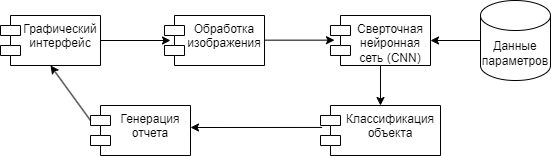
\includegraphics[width=1\linewidth]{comp}}
\caption{Диаграмма компонентов}
\label{comp:image}
\end{figure}

